\documentclass[a4paper]{article}
\usepackage[]{graphicx}\usepackage[]{color}
% maxwidth is the original width if it is less than linewidth
% otherwise use linewidth (to make sure the graphics do not exceed the margin)
\makeatletter
\def\maxwidth{ %
  \ifdim\Gin@nat@width>\linewidth
    \linewidth
  \else
    \Gin@nat@width
  \fi
}
\makeatother

\definecolor{fgcolor}{rgb}{0.345, 0.345, 0.345}
\newcommand{\hlnum}[1]{\textcolor[rgb]{0.686,0.059,0.569}{#1}}%
\newcommand{\hlstr}[1]{\textcolor[rgb]{0.192,0.494,0.8}{#1}}%
\newcommand{\hlcom}[1]{\textcolor[rgb]{0.678,0.584,0.686}{\textit{#1}}}%
\newcommand{\hlopt}[1]{\textcolor[rgb]{0,0,0}{#1}}%
\newcommand{\hlstd}[1]{\textcolor[rgb]{0.345,0.345,0.345}{#1}}%
\newcommand{\hlkwa}[1]{\textcolor[rgb]{0.161,0.373,0.58}{\textbf{#1}}}%
\newcommand{\hlkwb}[1]{\textcolor[rgb]{0.69,0.353,0.396}{#1}}%
\newcommand{\hlkwc}[1]{\textcolor[rgb]{0.333,0.667,0.333}{#1}}%
\newcommand{\hlkwd}[1]{\textcolor[rgb]{0.737,0.353,0.396}{\textbf{#1}}}%
\let\hlipl\hlkwb

\usepackage{framed}
\makeatletter
\newenvironment{kframe}{%
 \def\at@end@of@kframe{}%
 \ifinner\ifhmode%
  \def\at@end@of@kframe{\end{minipage}}%
  \begin{minipage}{\columnwidth}%
 \fi\fi%
 \def\FrameCommand##1{\hskip\@totalleftmargin \hskip-\fboxsep
 \colorbox{shadecolor}{##1}\hskip-\fboxsep
     % There is no \\@totalrightmargin, so:
     \hskip-\linewidth \hskip-\@totalleftmargin \hskip\columnwidth}%
 \MakeFramed {\advance\hsize-\width
   \@totalleftmargin\z@ \linewidth\hsize
   \@setminipage}}%
 {\par\unskip\endMakeFramed%
 \at@end@of@kframe}
\makeatother

\definecolor{shadecolor}{rgb}{.97, .97, .97}
\definecolor{messagecolor}{rgb}{0, 0, 0}
\definecolor{warningcolor}{rgb}{1, 0, 1}
\definecolor{errorcolor}{rgb}{1, 0, 0}
\newenvironment{knitrout}{}{} % an empty environment to be redefined in TeX

\usepackage{alltt}
\newcommand{\SweaveOpts}[1]{}  % do not interfere with LaTeX
\newcommand{\SweaveInput}[1]{} % because they are not real TeX commands
\newcommand{\Sexpr}[1]{}       % will only be parsed by R




\usepackage[utf8]{inputenc}
%\usepackage[ngerman]{babel}
\usepackage{a4wide,paralist}
\usepackage{amsmath, amssymb, xfrac, amsthm}
\usepackage{dsfont}
\usepackage[usenames,dvipsnames]{xcolor}
\usepackage{amsfonts}
\usepackage{graphicx}
\usepackage{caption}
\usepackage{subcaption}
\usepackage{framed}
\usepackage{multirow}
\usepackage{bytefield}
\usepackage{csquotes}
\usepackage[breakable, theorems, skins]{tcolorbox}
\usepackage{hyperref}
\usepackage{cancel}
\usepackage{bm}


\input{../../style/common}

\tcbset{enhanced}

\DeclareRobustCommand{\mybox}[2][gray!20]{%
	\iffalse
	\begin{tcolorbox}[   %% Adjust the following parameters at will.
		breakable,
		left=0pt,
		right=0pt,
		top=0pt,
		bottom=0pt,
		colback=#1,
		colframe=#1,
		width=\dimexpr\linewidth\relax,
		enlarge left by=0mm,
		boxsep=5pt,
		arc=0pt,outer arc=0pt,
		]
		#2
	\end{tcolorbox}
	\fi
}

\DeclareRobustCommand{\myboxshow}[2][gray!20]{%
%	\iffalse
	\begin{tcolorbox}[   %% Adjust the following parameters at will.
		breakable,
		left=0pt,
		right=0pt,
		top=0pt,
		bottom=0pt,
		colback=#1,
		colframe=#1,
		width=\dimexpr\linewidth\relax,
		enlarge left by=0mm,
		boxsep=5pt,
		arc=0pt,outer arc=0pt,
		]
		#2
	\end{tcolorbox}
%	\fi
}


%exercise numbering
\renewcommand{\theenumi}{(\alph{enumi})}
\renewcommand{\theenumii}{\roman{enumii}}
\renewcommand\labelenumi{\theenumi}


\font \sfbold=cmssbx10

\setlength{\oddsidemargin}{0cm} \setlength{\textwidth}{16cm}


\sloppy
\parindent0em
\parskip0.5em
\topmargin-2.3 cm
\textheight25cm
\textwidth17.5cm
\oddsidemargin-0.8cm
\pagestyle{empty}

\newcommand{\kopf}[1] {
\hrule
\vspace{.15cm}
\begin{minipage}{\textwidth}
%akwardly i had to put \" here to make it compile correctly
	{\sf\bf Introduction to Machine Learning \hfill Exercise sheet #1\\
	 \url{https://introduction-to-machine-learning.netlify.app/} \hfill WiSe 2020/2021}
\end{minipage}
\vspace{.05cm}
\hrule
\vspace{1cm}}

\newenvironment{allgemein}
	{\noindent}{\vspace{1cm}}

\newcounter{aufg}
\newenvironment{aufgabe}
	{\refstepcounter{aufg}\textbf{Exercise \arabic{aufg}:}\\ \noindent}
	{\vspace{0.5cm}}

\newcounter{loes}
\newenvironment{loesung}
	{\refstepcounter{loes}\textbf{Solution \arabic{loes}:}\\\noindent}
	{\bigskip}
	
\newenvironment{bonusaufgabe}
	{\refstepcounter{aufg}\textbf{Exercise \arabic{aufg}*\footnote{This
	is a bonus exercise.}:}\\ \noindent}
	{\vspace{0.5cm}}

\newenvironment{bonusloesung}
	{\refstepcounter{loes}\textbf{Solution \arabic{loes}*:}\\\noindent}
	{\bigskip}



\begin{document}
% !Rnw weave = knitr



\input{../../latex-math/basic-math.tex}
\input{../../latex-math/basic-ml.tex}

\kopf{4}

\loesung{

See \href{https://github.com/compstat-lmu/lecture_i2ml/blob/master/exercises/supervised-classification/sol_mlr_dec_boundaries.R}{R code}
}

\dlz
\loesung{

\begin{enumerate}
\item[a)] $k = 3$

2 circles and 1 triangle, so our point is also a circle

\begin{knitrout}
\definecolor{shadecolor}{rgb}{0.969, 0.969, 0.969}\color{fgcolor}

{\centering 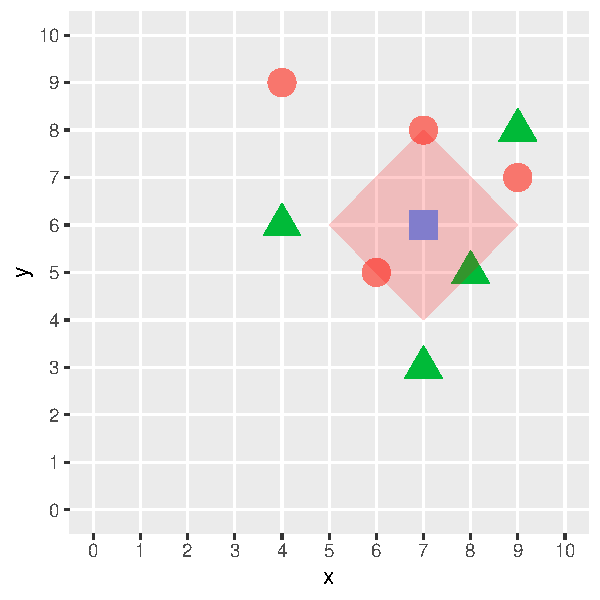
\includegraphics[width=\maxwidth]{figure/unnamed-chunk-3-1} 

}


\end{knitrout}

\item[b)] $k = 5$

3 circles and 3 triangles, we have to specify beforehand what to do in case of a tie

\begin{knitrout}
\definecolor{shadecolor}{rgb}{0.969, 0.969, 0.969}\color{fgcolor}

{\centering 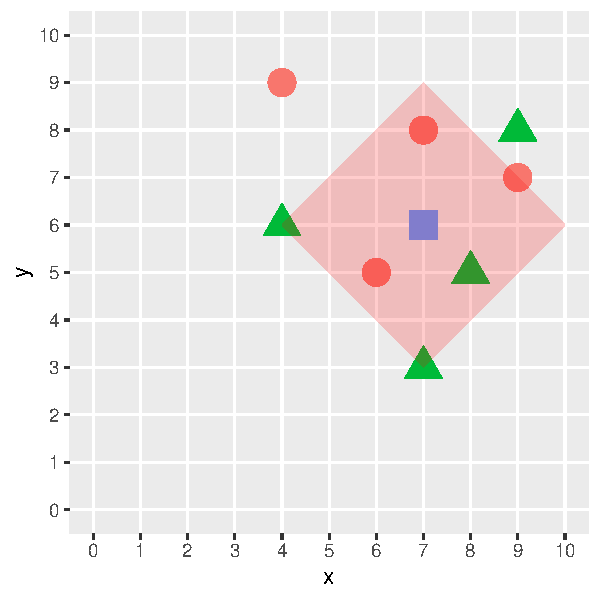
\includegraphics[width=\maxwidth]{figure/unnamed-chunk-4-1} 

}


\end{knitrout}

\item[c)] $k = 7$

3 circles and 4 triangles, so our point is also a triangle

\begin{knitrout}
\definecolor{shadecolor}{rgb}{0.969, 0.969, 0.969}\color{fgcolor}

{\centering 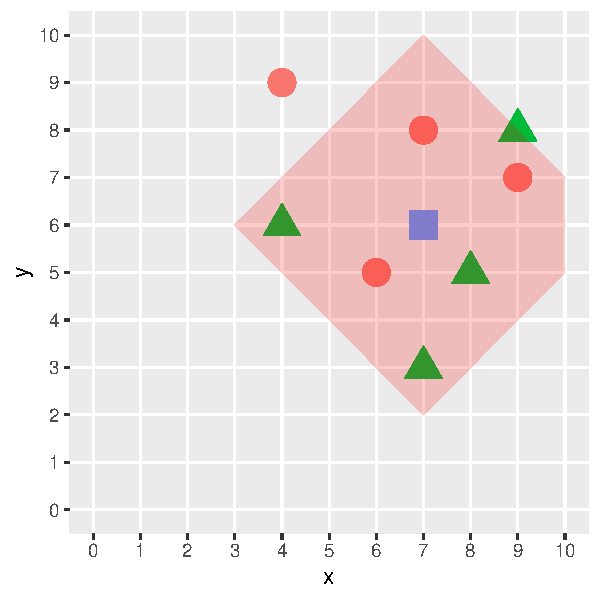
\includegraphics[width=\maxwidth]{figure/unnamed-chunk-5-1} 

}


\end{knitrout}

\end{enumerate}


  
}

\newpage

\dlz
\loesung{

\begin{enumerate}

  \item[a)]

When using the naive Bayes classifier, the features $x := (x_\text{Color},x_\text{Form},x_\text{Origin})$ given the category $y \in \{\text{yes},\text{no}\}$ are assumed to be conditionally independent of each other, s.t.

$$p((x_\text{Color},x_\text{Form},x_\text{Origin})|y = k) = p(x_\text{Color}|y = k)\cdot p(x_\text{Form}|y = k) \cdot p(x_\text{Origin}|y = k).$$

For the posterior probabilities $\pi_k(x)$ it holds that
\begin{align*} \pi_k(x) \propto & \; \underbrace{\pi_k \cdot p(x_\text{Color}|y = k)\cdot p(x_\text{Form}|y = k) \cdot p(x_\text{Origin}|y = k)}_{=: \alpha_k(x)} \\
\iff & \exists c \in \mathbb{R}: \pi_k(x) = c \cdot \alpha_k(x),\end{align*}
where $\pi_k$ is the prior probability of class $k$.
From this and since the posterior probabilities need to sum up to 1, it holds that 
\begin{align*}1 =& \; c \cdot \alpha_\text{yes}(x) +  c \cdot \alpha_\text{no}(x)\\
\iff & c = \frac{1}{\alpha_\text{yes}(x) + \alpha_\text{no}(x)}.
\end{align*}
This means in order to compute $\pi_\text{yes}(x)$ the scores $\alpha_\text{yes}(x)$ and $\alpha_\text{no}(x)$ are needed.\\ Now we want to compute for a new fruit the posterior probability $\hat{\pi}_{yes}((\text{yellow},\text{round},\text{imported}))$. \\
Note that we do not know the \emph{true} prior probability and the \emph{true} conditional densities. Here -since the target and the features are categorical- we can estimate them with the relative frequencies encountered in the data, s.t.
\begin{align*}
\hat{\alpha}_\text{yes}(x) = & \;  \hat{\pi}_{yes} \cdot \hat{p}(\text{yellow}|y = \text{yes})\cdot \hat{p}(\text{round}|y = \text{yes}) \cdot \hat{p}(\text{imported}|y = \text{yes}) \\
= & \; \hat{\P}(y = \text{yes}) \cdot \hat{\P}(x_\text{Color} = \text{yellow}|y = \text{yes})\cdot \hat{\P}(x_\text{Form}=\text{round}|y = \text{yes}) \cdot \hat{\P}(x_\text{Origin}=\text{imported}|y = \text{yes}) \\
= & \; \frac{3}{8} \cdot \frac{1}{3} \cdot \frac{1}{3} \cdot 1 = \frac{1}{24} \approx 0.042, \\
\hat{\alpha}_\text{no}(x) = & \;  \hat{\pi}_{no} \cdot \hat{p}(\text{yellow}|y = \text{no})\cdot \hat{p}(\text{round}|y = \text{no}) \cdot \hat{p}(\text{imported}|y = \text{no}) \\
= & \; \hat{\P}(y = \text{no}) \cdot \hat{\P}(x_\text{Color} = \text{yellow}|y = \text{no})\cdot \hat{\P}(x_\text{Form}=\text{round}|y = \text{no}) \cdot \hat{\P}(x_\text{Origin}=\text{imported}|y = \text{no}) \\
= & \; \frac{5}{8} \cdot \frac{2}{5} \cdot \frac{3}{5} \cdot \frac{2}{5} = \frac{3}{50} = 0.06.
\end{align*}
At this stage we can already see that the predicted label is "no", since $ \hat{\alpha}_\text{no}(x) = 0.06>\frac{1}{24} = 
\hat{\alpha}_\text{yes}(x)$. \\
With this we can calculate the posterior probability
$$\hat{\pi}_\text{yes}(x) = \frac{\hat{\alpha}_\text{yes}(x)}{\hat{\alpha}_\text{yes}(x) + \hat{\alpha}_\text{no}(x)} \approx 0.41.$$


    Corresponding \texttt{R}-Code:

\begin{knitrout}
\definecolor{shadecolor}{rgb}{0.969, 0.969, 0.969}\color{fgcolor}\begin{kframe}
\begin{alltt}
\hlstd{df_banana} \hlkwb{<-} \hlkwd{data.frame}\hlstd{(}
  \hlkwc{Color} \hlstd{=} \hlkwd{as.factor}\hlstd{(}
    \hlkwd{c}\hlstd{(}\hlstr{"yellow"}\hlstd{,} \hlstr{"yellow"}\hlstd{,} \hlstr{"yellow"}\hlstd{,} \hlstr{"brown"}\hlstd{,} \hlstr{"brown"}\hlstd{,} \hlstr{"green"}\hlstd{,} \hlstr{"green"}\hlstd{,} \hlstr{"red"}\hlstd{)),}
  \hlkwc{Form} \hlstd{=} \hlkwd{as.factor}\hlstd{(}
    \hlkwd{c}\hlstd{(}\hlstr{"oblong"}\hlstd{,} \hlstr{"round"}\hlstd{,} \hlstr{"oblong"}\hlstd{,} \hlstr{"oblong"}\hlstd{,} \hlstr{"round"}\hlstd{,} \hlstr{"round"}\hlstd{,} \hlstr{"oblong"}\hlstd{,} \hlstr{"round"}\hlstd{)),}
  \hlkwc{Origin} \hlstd{=} \hlkwd{as.factor}\hlstd{(}
    \hlkwd{c}\hlstd{(}\hlstr{"imported"}\hlstd{,} \hlstr{"domestic"}\hlstd{,} \hlstr{"imported"}\hlstd{,} \hlstr{"imported"}\hlstd{,} \hlstr{"domestic"}\hlstd{,} \hlstr{"imported"}\hlstd{,}
    \hlstr{"domestic"}\hlstd{,} \hlstr{"imported"}\hlstd{)),}
  \hlkwc{Banana} \hlstd{=} \hlkwd{as.factor}\hlstd{(}\hlkwd{c}\hlstd{(}\hlstr{"yes"}\hlstd{,} \hlstr{"no"}\hlstd{,} \hlstr{"no"}\hlstd{,} \hlstr{"yes"}\hlstd{,} \hlstr{"no"}\hlstd{,} \hlstr{"yes"}\hlstd{,} \hlstr{"no"}\hlstd{,} \hlstr{"no"}\hlstd{))}
\hlstd{)}

\hlstd{new_fruit} \hlkwb{<-} \hlkwd{data.frame}\hlstd{(}\hlkwc{Color} \hlstd{=} \hlstr{"yellow"}\hlstd{,} \hlkwc{Form} \hlstd{=} \hlstr{"round"}\hlstd{,} \hlkwc{Origin} \hlstd{=} \hlstr{"imported"}\hlstd{,} \hlkwc{Banana} \hlstd{=} \hlnum{NA}\hlstd{)}
\hlstd{df_banana} \hlkwb{<-} \hlkwd{rbind}\hlstd{(df_banana, new_fruit)}

\hlkwd{library}\hlstd{(mlr3)}
\hlkwd{library}\hlstd{(mlr3learners)}

\hlstd{nb_learner} \hlkwb{<-} \hlkwd{lrn}\hlstd{(}\hlstr{"classif.naive_bayes"}\hlstd{,}
                  \hlkwc{predict_type} \hlstd{=} \hlstr{"prob"}\hlstd{)}

\hlstd{banana_task} \hlkwb{<-} \hlstd{TaskClassif}\hlopt{$}\hlkwd{new}\hlstd{(}
  \hlkwc{id} \hlstd{=} \hlstr{"banana"}\hlstd{,}
  \hlkwc{backend} \hlstd{= df_banana,}
  \hlkwc{target} \hlstd{=} \hlstr{"Banana"}
\hlstd{)}

\hlstd{nb_learner}\hlopt{$}\hlkwd{train}\hlstd{(banana_task,} \hlkwc{row_ids}\hlstd{=}\hlnum{1}\hlopt{:}\hlnum{8}\hlstd{)}

\hlstd{nb_learner}\hlopt{$}\hlkwd{predict}\hlstd{(banana_task,} \hlkwc{row_ids} \hlstd{=} \hlnum{9}\hlstd{)}
\end{alltt}
\begin{verbatim}
## <PredictionClassif> for 1 observations:
##  row_ids truth response   prob.no  prob.yes
##        9  <NA>       no 0.5901639 0.4098361
\end{verbatim}
\end{kframe}
\end{knitrout}

  \item[b)]
    For the distribution of a numerical feature given the the category we need to specify a probability distribution with continuous support.
    For example, for the information $x_\text{Length}$ we could assume that $p(x_\text{Length} | y = \text{yes}) \sim \mathcal{N}(\mu_\text{yes},\sigma^2_\text{yes})$ and $p(x_\text{Length} | y = \text{no}) \sim \mathcal{N}(\mu_\text{no},\sigma^2_\text{no})$. (To estimate these normal distributions one would need to estimate their parameters $\mu_\text{yes},\mu_\text{no},\sigma^2_\text{yes},\sigma^2_\text{no}$ on the data respectively)
\end{enumerate}
}


\end{document}
